%author: Simone Notargiacomo, Lorenzo Tavernese, Ibrahim Khalili
%date: 19 Giugno 2008
\documentclass[a4paper,italian,12pt]{beamer}
\usepackage[utf8]{inputenc}
\usepackage[italian,english]{babel}
\usepackage[T1]{fontenc}
\usepackage{beamerthemesplit}
\usepackage{graphicx}
\usepackage{float}
\usepackage{xcolor}
\usepackage{times}
\usepackage{colortbl}

\setbeamercolor{uppercol}{fg=black,bg=white}
\setbeamercolor{lowercol}{fg=black,bg=blue}

%\usepackage{tikz}
%\usetikzlibrary{arrows}
%\tikzstyle{block}=[draw opacity=0.7,line width=1.4cm]

%\setbeamercolor{sidebar right}{bg=black!15}
%\setbeamercolor{structure}{fg=blue}
%\setbeamercolor{author}{parent=structure}

\usetheme{Antibes}
\useoutertheme{smoothbars}
%\useoutertheme{infolines}
%\usecolortheme{rose}
\useinnertheme{circles}

\title{Ingegneria del Web 07/08}
\institute{Università di Roma Tor Vergata}
\author{Ibrahim Khalili}
%\logo{
\includegraphics[scale=0.1]{etc/tortellalogo.jpg}}
\date{\today}

\begin{document}
	\begin{frame}
		\titlepage
		\begin{figure}[H]
			\begin{center}
				
\includegraphics[scale=0.4]{etc/tortellalogo.jpg}
			\end{center}
		\end{figure}
	\end{frame}

    \section{Sommario}
	    \frame{\tableofcontents}

    \section{TorTella}
    	\subsection{Introduzione}
    		\begin{frame}
    			\frametitle{Caratteristiche}
    			\begin{itemize}
    				\item Sistema completamente decentralizzato per lo scambio di messaggi tra utenti.
					\vspace{2mm}    				
    				\item Meccanismo di invio dei pacchetti tramite flooding.
					\vspace{2mm}    				
    				\item Controllo dei pacchetti duplicati.
					\vspace{2mm}    				
    				\item Pacchetti trasportati nel campo dati del protocollo HTTP. 
    			\end{itemize}
    		\end{frame}
    	\subsection{Protocollo}
    		\begin{frame}
    			\frametitle{Definizione}
   				\begin{beamerboxesrounded}[upper=palette primary,lower=palette primary,shadow=true]{ }
    				TorTella nasce dal protocollo Gnutella, da cui prende alcune idee e ne introduce altre
    			\end{beamerboxesrounded}
				\vspace{10mm}
    			\begin{itemize}
    				\item Pacchetto PING non viaggia in flooding.
    				\item Diminuzione carico rete.
    				\item Realizzati nuovi descrittori.
    				\item TTL e HOPS presenti solo in alcuni pacchetti.
    				\item Utilizzo del Backward Routing.
    			\end{itemize}
    		\end{frame}
    		\begin{frame}
    			\frametitle{Descrittori}	
	    			\textbf{Header TorTella}
    				\begin{figure}[H]
						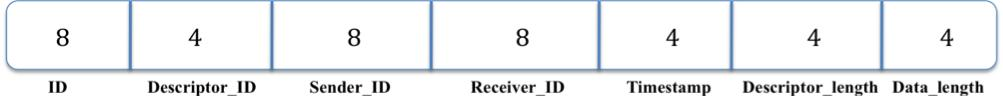
\includegraphics[scale=0.15]{etc/tortellaheader.jpg}
					\end{figure}
					\textbf{Ping Descriptor}: Utilizzato per la ricerca degli host sulla rete
    				\begin{figure}[H]
						
\includegraphics[scale=0.3]{etc/ping.jpg}
					\end{figure}
					\textbf{Join Descriptor}: Utilizzato per l'accesso ad una chat
    				\begin{figure}[H]
						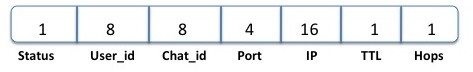
\includegraphics[scale=0.3]{etc/join.jpg}
					\end{figure}
    		\end{frame}
    		\begin{frame}
    			\frametitle{Descrittori}
	    			\textbf{Search Descriptor}: Utilizzato per la ricerca di chat
    				\begin{figure}[H]
						
\includegraphics[scale=0.3]{etc/search.jpg}
					\end{figure}					
					\textbf{SearchHits Descriptor}: Utilizzato per contenere i risultati ottenuti dal SEARCH
    				\begin{figure}[H]
						
\includegraphics[scale=0.3]{etc/searchhits.jpg}
					\end{figure}					
					\textbf{Leave Descriptor}: Utilizzato per abbandonare una chat
    				\begin{figure}[H]
						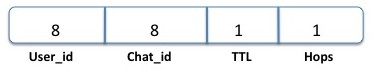
\includegraphics[scale=0.3]{etc/leave.jpg}
					\end{figure}
			\end{frame}
	
%    	\subsection{Conversione dati}
%    		\begin{frame}
%    			\frametitle{Funzioni di parsing}
%    			\begin{itemize}
%    				\item
	\section{Socket}
		\subsection{Connessioni}
			\begin{frame}
				\frametitle{Parametri e Configurazioni}
				\begin{itemize}
					\item Utilizzo di connessioni persistenti (SO\_KEEPALIVE).
						\begin{itemize}
							\vspace{2mm}
							\item Necessario per evitare l'instaurazione di una nuova connessione ad ogni invio di un pacchetto.
							\item Riduzione sensibile della latenza e dell'overhead.							 
						\end{itemize}
					\vspace{5mm}	
					\item Modifica del comportamento della \texttt{bind()} per il riutilizzo di indirizzi locali (SO\_REUSEADDR).
						\begin{itemize}
							\vspace{2mm}
							\item Utile in caso di crash del'applicazione.
							\item In caso di riavvio dell'applicazione.
						\end{itemize}
				\end{itemize}
			\end{frame}	
		\subsection{Scambio dei messaggi}
			\begin{frame}
				\frametitle{Invio e Ricezione}
					\begin{itemize}
						\item Messaggi inviati tramite chiamata di sistema \texttt{write()}.
						\vspace{5mm}
						\item Ricezione di messaggi di qualsiasi dimensione. 
						\item Utilizzo di un buffer con memoria dinamica.
						\item Possibilità di ricezione di file.
					\end{itemize}	
			\end{frame}
	\section{Failure Detection}
		\subsection{Timer Thread}
			\begin{frame}
				\frametitle{Descrizione}
				\begin{itemize}
					\item Lanciato il Timer Thread che gestisce il meccanismo di Failure Detection.
					\item Effettuato il controllo tramite l'invio di pacchetti PING a tutti i vicini.
					\item Controllo effettuato ad intervalli di tempo predefiniti.
					\item Mancata risposta indica failure del peer remoto.
					\item Se c'è mancata risposta si elimina il peer dalle proprie stutture dati.
				\end{itemize}
			\end{frame}
			\begin{frame}
				\frametitle{Esempio}
				\begin{figure}[H]
					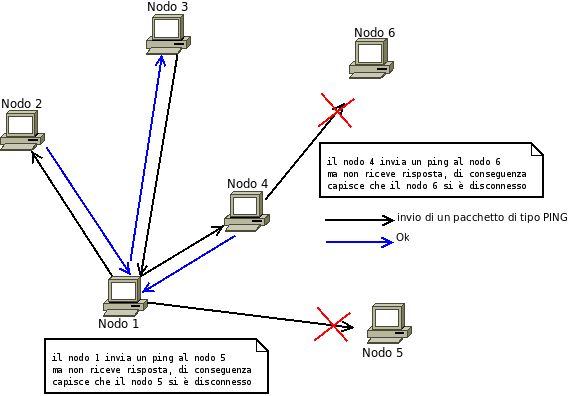
\includegraphics[scale=0.3]{etc/failure_detection.png}
				\end{figure}
			\end{frame}
\end{document}